\section{Comparison of NLP Transformer Models}
\label{sxn:nlp}

In the past two years, nearly 100 open source, pre-trained DNNs for Natural Language Processing (NLP) have emerged,
based on the revolutionary Transformer architecture, including variants of BERT, Transformer-XML, GPT, etc.
The Transformer architectures consist of blocks of Attention layers, containing of 2 large, Feed Forward (Linear)
weight matrics \cite{Attn2017}. In contrast to the smaller pre-Activation maps arising in Cond2D layers,
the Attention matrices ar

\paragraph{GPT vs GPT2}
Here, we use the \emph{WeightWatcher} tool to analyze the OpenAI GPT and GPT2 models, which gives us
the opportunity to analyze the effect of both training the same model with different size data sets,
These GPT models have generated significant media attention because of its remarkable ability to
 generate fake text, and it's potential misuse. 
The original GPT and later GPT model have the same architecture and number of layers, but
the original GPT was released having been trained on a deficient data set.  Recently,
 however, a much improved GPT2 model has been released, which is remarkably good at creating 
auto-genetated text.  

\charles{more here ?}
We analyze GPT models deployed with the popular HuggingFace PyTorch library.
GPT has 12 layers, with 4 Multi-head Attention Blocks, giving $48$ Layer Weight Matrices $\mathbf{W}$.
Each Block has 2 components, the Self Attention (attn) and the Projection (proj) matrics.  
The self-attention  matrices are larger, of dimension ($2304\times 768$) or ($3072\times 768$).
The projection layer concatenates the self-attention results into a vector (of dimension $768$).
This gives $50$ large, typically sparse weight matrices, and they can be
 \emph{poorly correlated} when trained with insufficient data--as we shall see below.

Because GPT and GPT are trained on different data sets, the initial Embedding matrices differ in shape.
GPT  has an initial Token and Positional Embedding layers, of dimension
$(40478\times 768)$ and $(512\times 768)$, resp, whereas GPT2 has input Embeddings of shape
$(50257\times 768)$ and $(1024\times 768)$, resp.  Interstingly, they also have very spectral properties,
also shown below.

The additional OpenAI GPT2 (English) models are: \emph{gpt-medium, got-large, and gpt-xl}, 
having include $12, 24, 36, and 48$ layers, resp., with increasingly larger weight matrices.
The model card for GPT2 is published on github.\footnote{\url{https://github.com/openai/gpt-2/blob/master/model_card.md}}.
Table \ref{table:nlp} reports results for the average log norm metrics, using \emph{weightwatcher (0.2.3)},
and with fully reproducible Jupyter notebooks.\footnote{\url{https://github.com/CalculatedContent/kdd2020}}


\begin{table}[t]
\small
\begin{center}
\begin{tabular}{|p{1in}|c|c|c|c|c|}
\hline
   &    & Frobenius Norm & Spectral Norm & Weighted Alpha & Alpha-Norm \\
 Series & \#Layers   & $\Vert\mathbf{W}\Vert_{F}$ & $\Vert\mathbf{W}\Vert_{\infty}$ & $\hat{\alpha}=\alpha\log\lambda_{max}$ & $\Vert\mathbf{X}\Vert^{\alpha}_{\alpha}$ \\
\hline
 GPT & & & & \\
 GPT2 (small) & & & & \\
 GPT2-medium & & & & \\
 GPT2-large & & & & \\
 GPT2-xl & & & & \\

\hline
\end{tabular}
\end{center}
\caption{Average Log Norm Metrics for pretrainnd OpenAI GPT and GPT2 models.}
\label{table:nlp}
\end{table}


\paragraph{The Heavy Tailed Power Law Exponents in GPT and GPT2}

are very differenmt, with GPT2 having both a notably smaller mean $\alpha$, and far fewer, unusually large outliers.
Figure \ref{fig:gpt-alphs-hist} shows the empirical density (histogram) of $\alpha$
for all layers in GPT (blue) and GPT2 (red).  \charles{discuss more}

\begin{figure}
   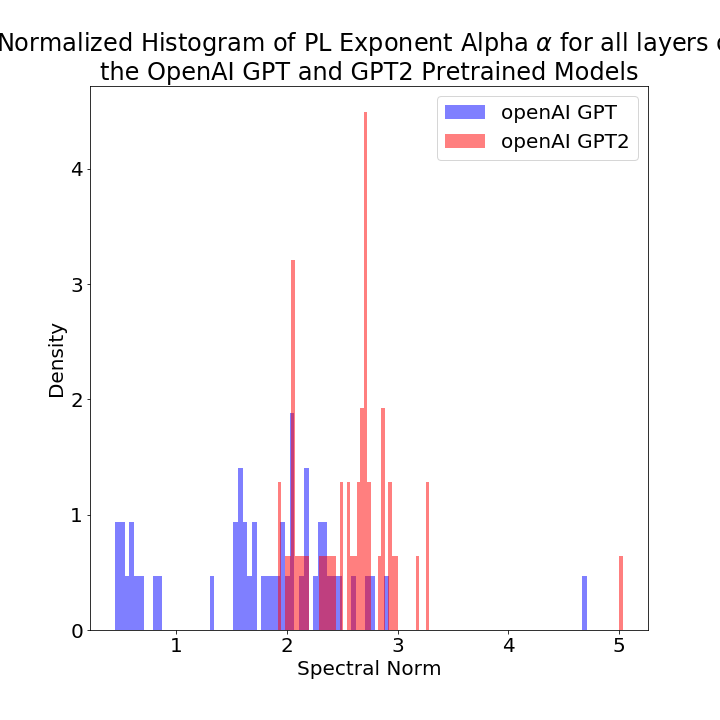
\includegraphics[scale=0.25]{img/gpt-alpha-hist.png}
   \caption{Comparison of heavy tailed power law exponent $\alpha$ for OpenAI GPT and GPT pretrained models}

   \label{fig:gpt-alphs-hist}
\end{figure}


\paragraph{The Correlation Flow in GPT and GPT2} also differs significantly between GPT and GPT2.
Figure \ref{fig:gpt-alpha-layer} plots $\alpha$ vs the layer id for each model.


\charles{Discuss Spectral Norm, alpha-Norm}

\begin{figure}[t]
    \centering

    \subfigure[ Power Law Exponent $\alpha$  ]{
        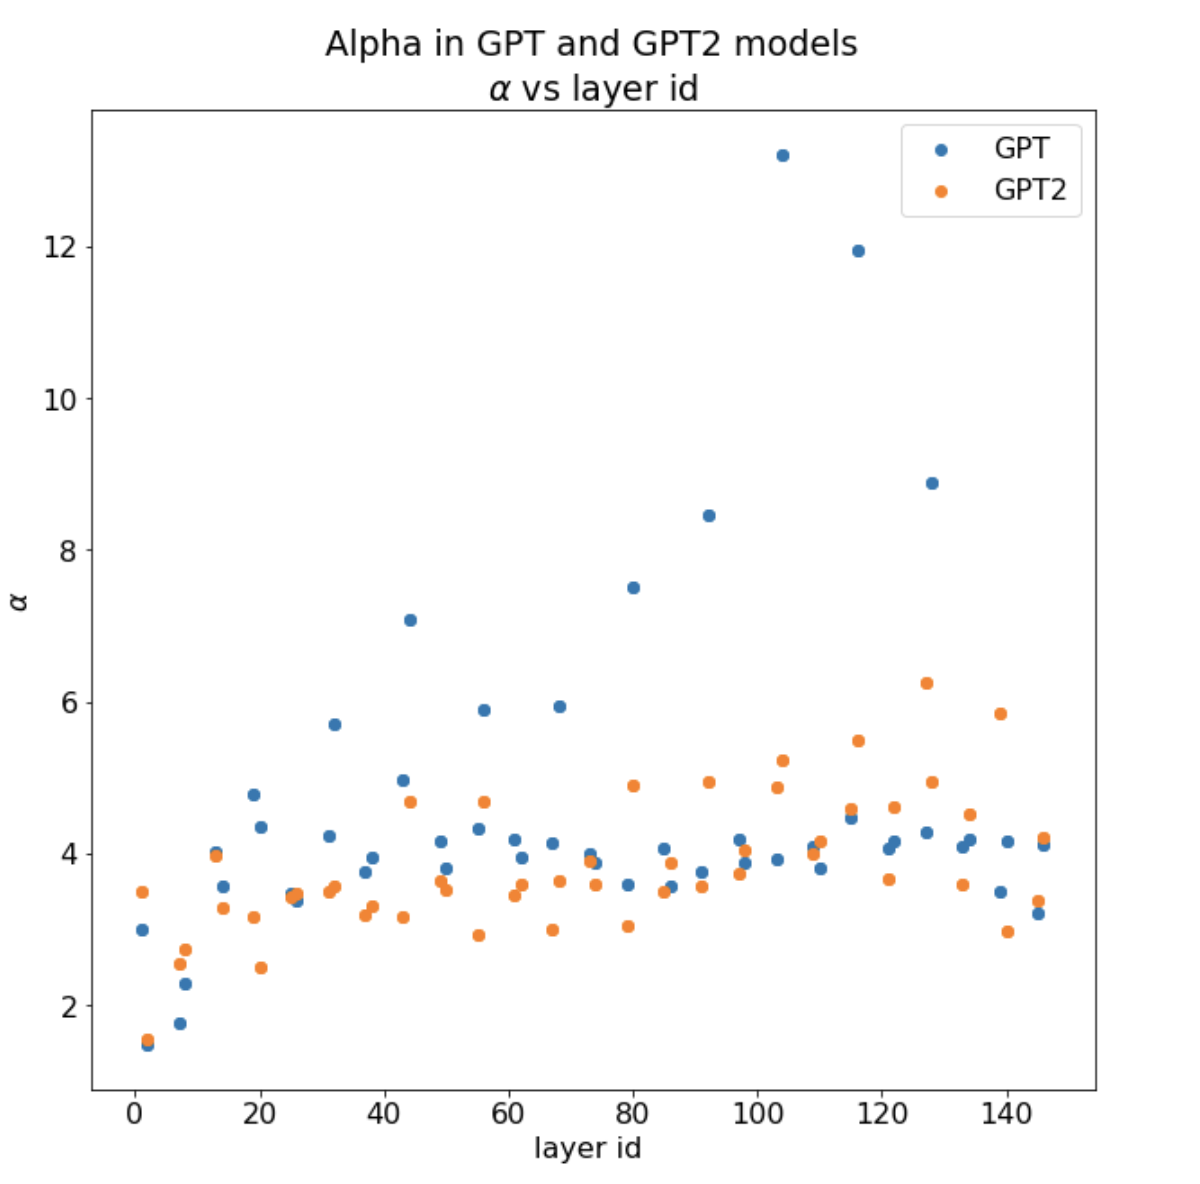
\includegraphics[width=4.0cm]{img/gpt-alpha-layer.png}
        \label{fig:gpt-alpha-layer}
    }
    \qquad
    \subfigure[ Spectral Norm $\Vert\mathbf{W}\Vert_{\infty}$]{
        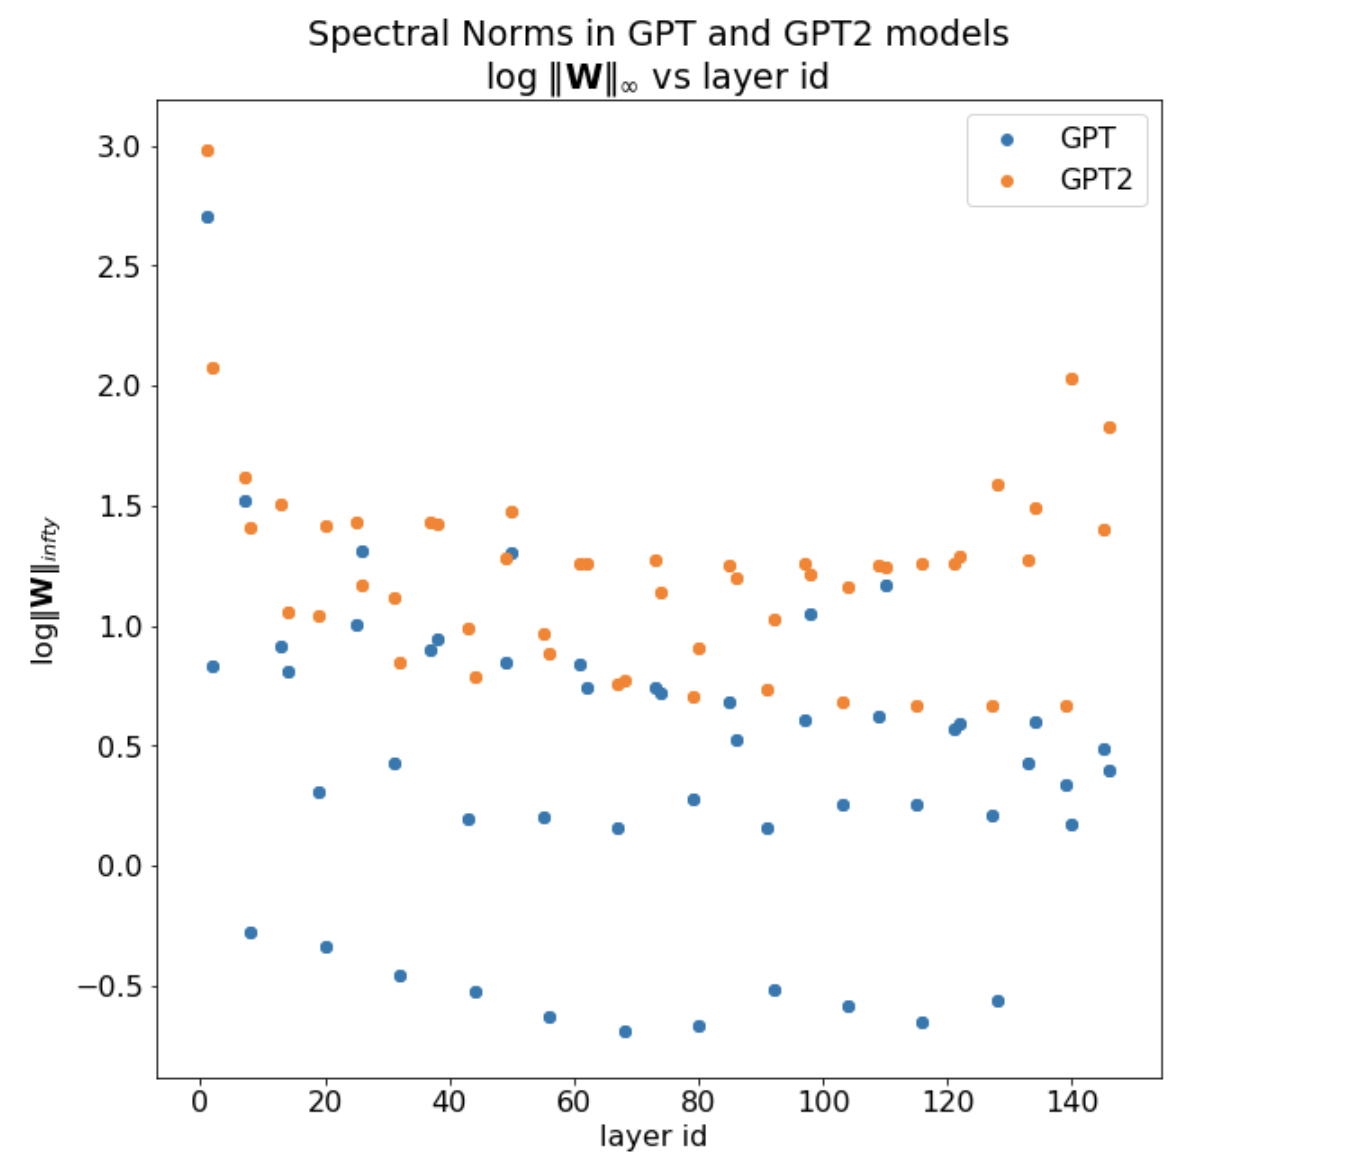
\includegraphics[width=4.5cm]{img/gpt-snorm-layer.png}
        \label{fig:resnet-snorm-layer}
    }
    \qquad
    \subfigure[ Alpha-Norm $\Vert\mathbf{X}\Vert_{\alpha}^{\alpha}$]{
        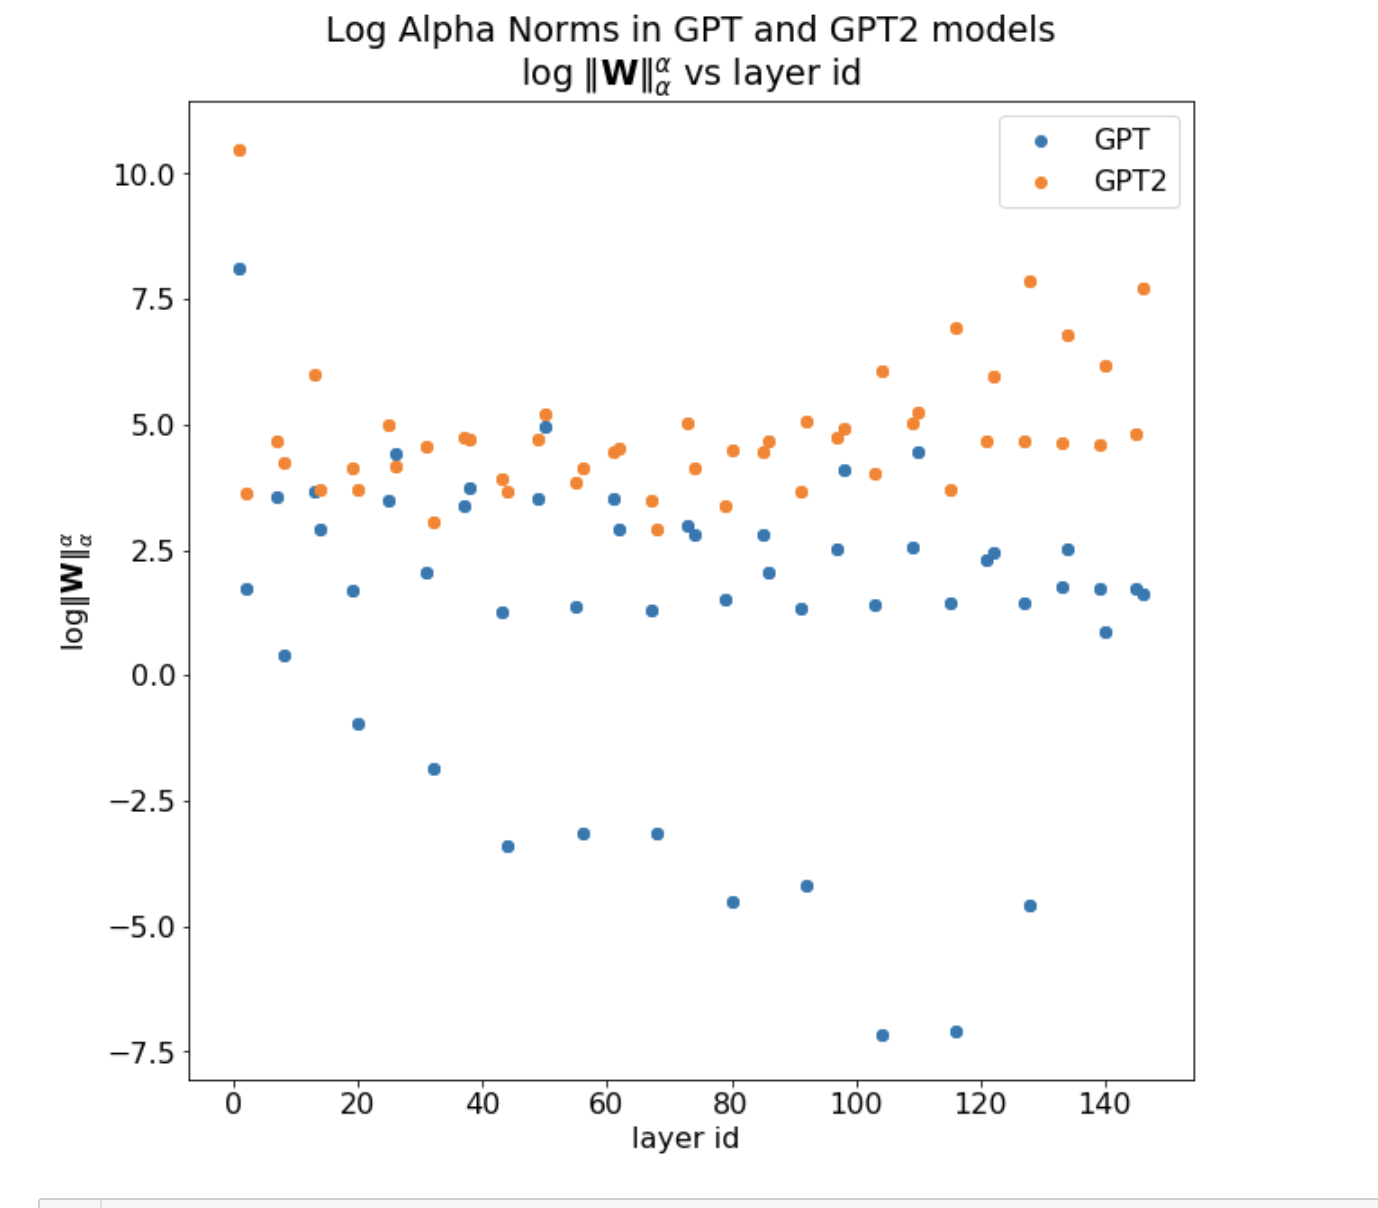
\includegraphics[width=4.5cm]{img/gpt-pnorm-layer.png}
        \label{fig:gpt-pnorm-layer}
    }
    \caption{Comparison of Correlation Flow and Spectral Norm for OpenAI GPT and GPT2   }
    \label{fig:gpt-alpha-layers}
\end{figure}

\paragraph{GPT2: small, medium, large, extra-large} 

Figure \ref{fig:gpt-alpha-layers} ...

For this series of GPT2 models, the average $\alpha$ still decreases with increasing model size,
althogh, the differences are less noticible than between the GPT and GPT2 models.
Unlike GPT, however, the Layer Spectral Norms $\vert\mathbf{W}\Vert_{\infty}$ 
and Alpha-Norms $\vert\mathbf{W}\Vert_{\alpha}^{\alpha}$
 behave  as expected for GPT2 layers, with the larger models 
consistently having  smaller norms. 

\begin{figure}[t]
    \centering

    \subfigure[ Power Law Exponent $\alpha$  ]{
        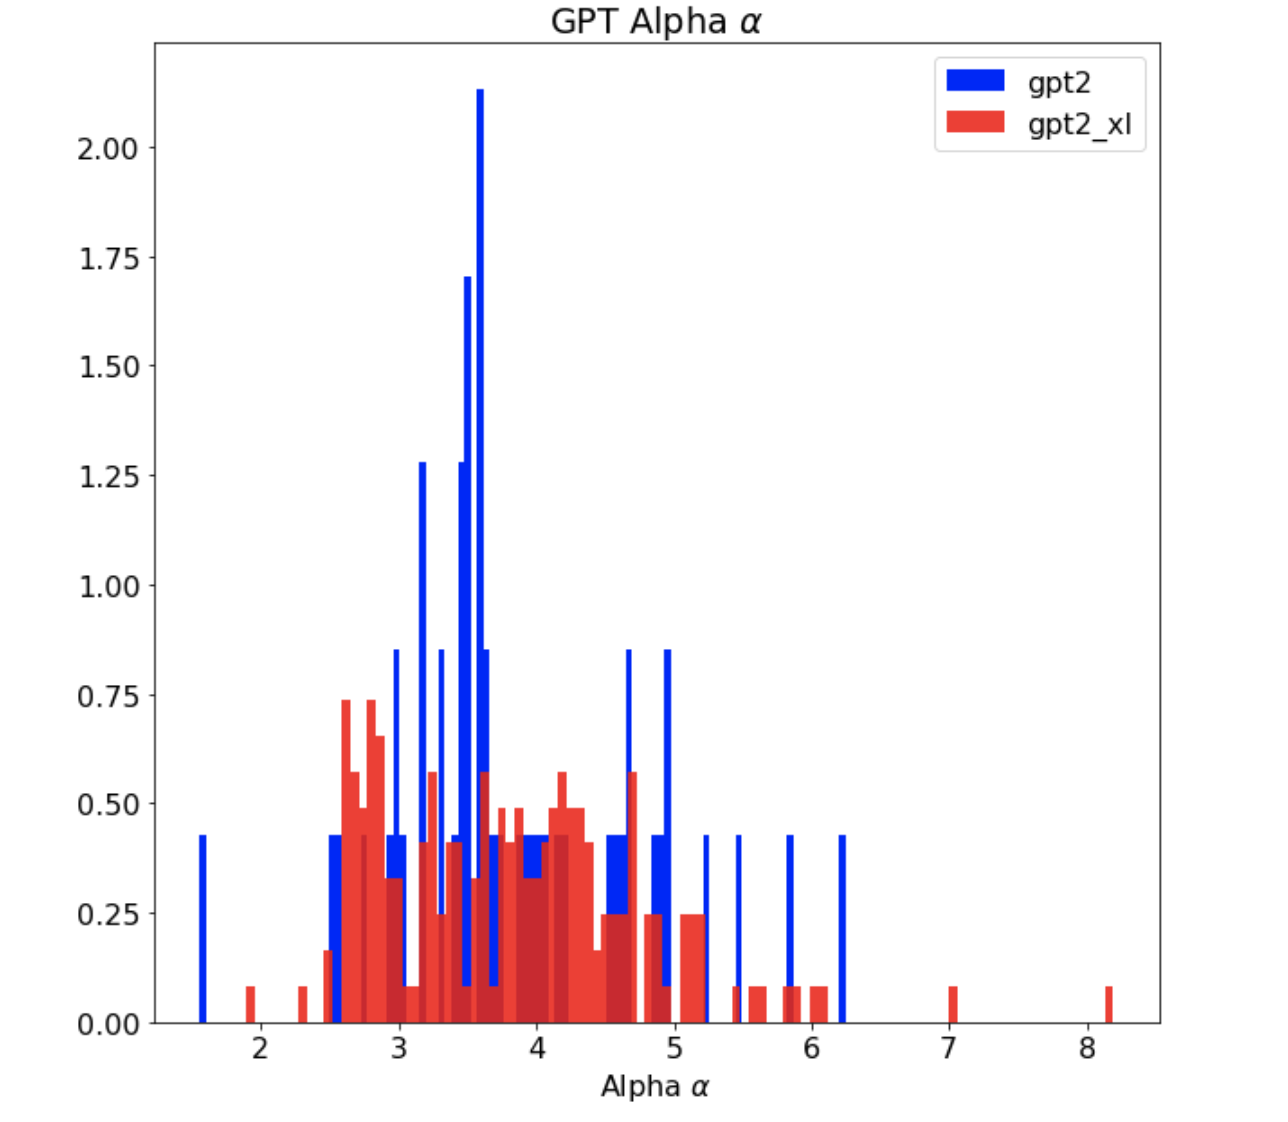
\includegraphics[width=4.5cm]{img/gpt2-alpha-hist.png}
        \label{fig:gpt-alpha-layer}
    }
    \qquad
    \subfigure[ Spectral Norm $\Vert\mathbf{W}\Vert_{\infty}$]{
        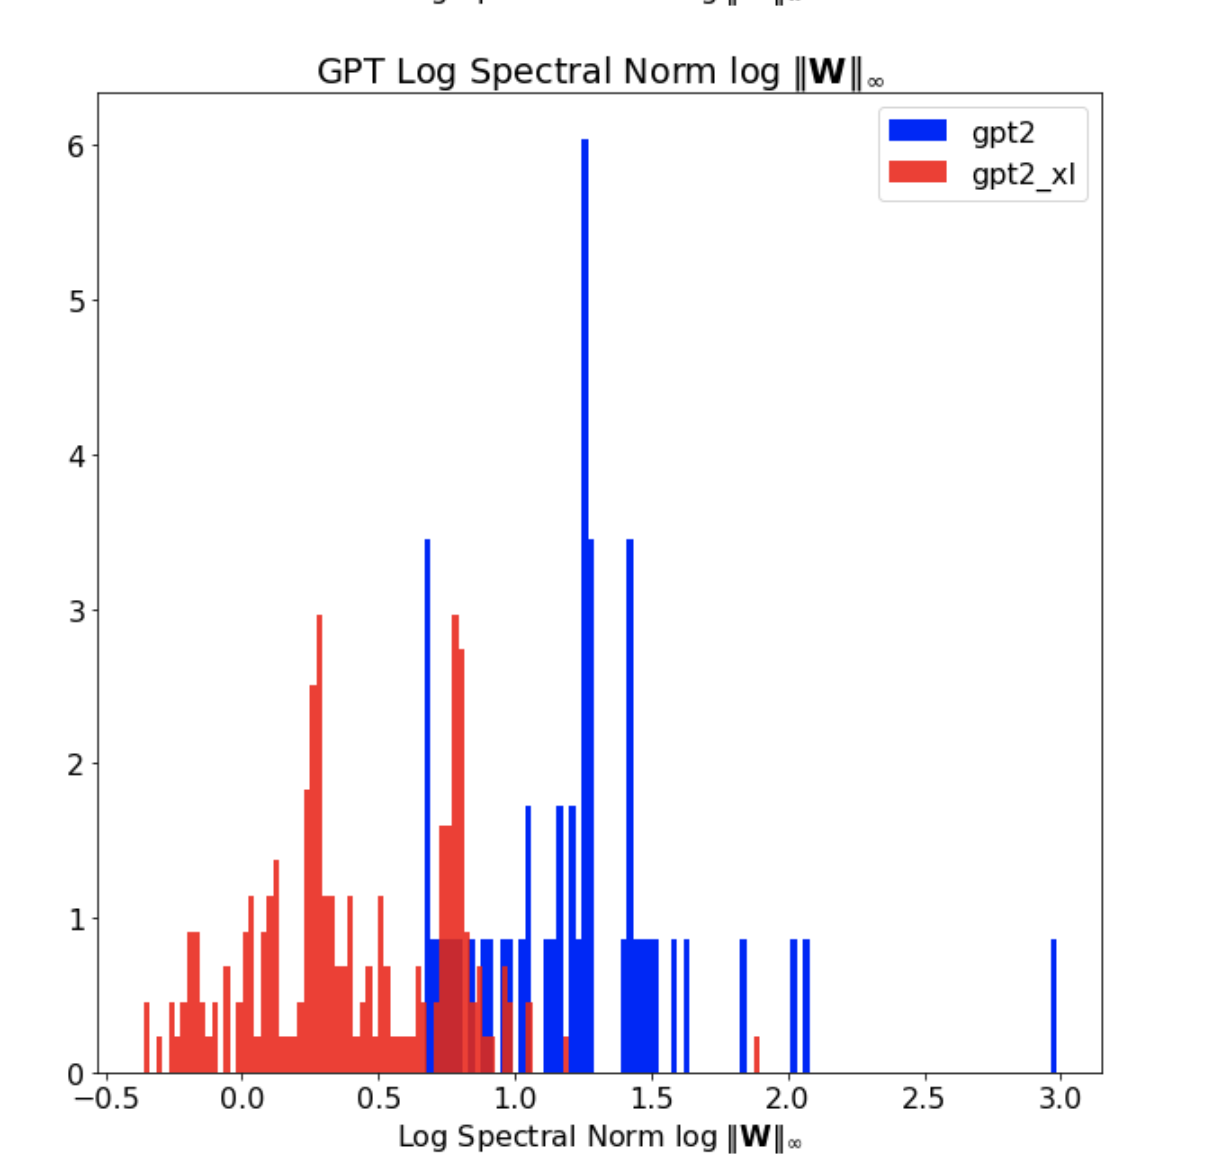
\includegraphics[width=4.5cm]{img/gpt2-snorm-hist.png}
        \label{fig:resnet-snorm-layer}
    }
    \qquad
    \subfigure[ Alpha-Norm $\Vert\mathbf{X}\Vert_{\alpha}^{\alpha}$]{
        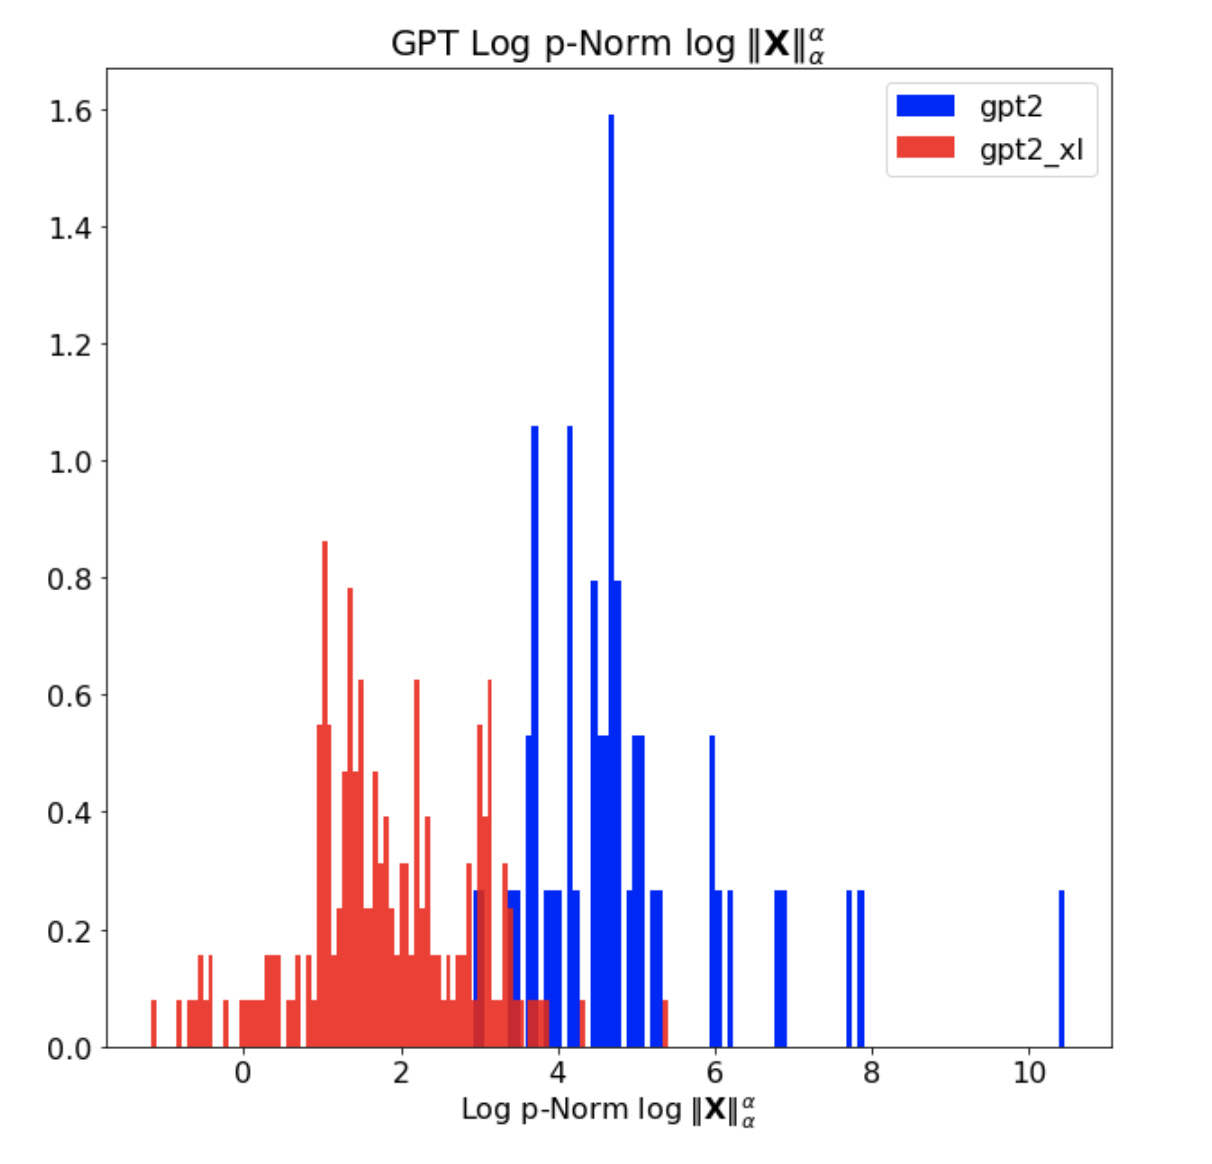
\includegraphics[width=4.5cm]{img/gpt2-pnorm-hist.png}
        \label{fig:gpt-pnorm-layer}
    }
    \caption{Comparison of Power Law Exponnents, Spectral Norm, and Alpha-Norm for different size models in the GPT2 architecture series.    }
    \label{fig:gpt-alpha-layers}
\end{figure}




